% !TEX TS-program = xelatex
% !BIB program = bibtex
% !TEX encoding = UTF-8 Unicode

\documentclass[
  twoside,
  % openright,
  openany,
  degree    = doctor,               % degree = master | doctor
  language  = english,              % language = chinese | english
  fontset   = template,             % fontset = default | template | system | overleaf
  watermark = true,                 % watermark = true | false
  doi       = true,                 % doi = true | false
  draftset = false,          % true for draft statement at cover, false for the final version
]{ntuthesis}

% !TeX root = ./main.tex

% --------------------------------------------------
% 資訊設定(Information Configs)
% --------------------------------------------------

\ntusetup{
  university*   = {National Taiwan University},
  university    = {國立臺灣大學},
  college       = {電機資訊學院},
  college*      = {College of Electrical Engineering and Computer Science},
  institute     = {光電工程學研究所},
  institute*    = {Graduate Institute of Photonics and Optoelectronics},
  title         = {基於矽光平台上之 O-band 1$\times$4 分波(解)多工濾波器},
  title*        = {O-band 1$\times$4 wavelength division (de)multiplexing filters on Silicon Photonics}, 
  author        = {鍾國方},
  author*       = {Kuo-Fang Chung},
  ID            = {D08941008},
  advisor       = {黃定洧},
  advisor*      = {Ding-Wei Huang},
  date          = {2022-09-26},         % 若註解掉,則預設為當天
  oral-date     = {2022-09-26},         % 若註解掉,則預設為當天
  DOI           = {10.5566/NTU2022XXXXX},
  keywords      = {矽光子, 陣列波導光柵, 波導布拉格光柵, 多模波導, 分波(解)多工器},
  keywords*     = {Silicon Photonics, waveguide Bragg grating, multi-mode waveguide, wavelength division (de)multiplexer},
}

% --------------------------------------------------
% 加載套件(Include Packages)
% --------------------------------------------------

% \usepackage[sort&compress]{natbib}      % 參考文獻
\usepackage[noadjust]{cite}     % replace with natbib

\usepackage{amsmath, amsthm, amssymb}   % 數學環境
\usepackage{ulem, CJKulem}              % 下劃線、雙下劃線與波浪紋效果
\usepackage{booktabs}                   % 改善表格設置
\usepackage{multirow}                   % 合併儲存格
\usepackage{diagbox}                    % 插入表格反斜線
\usepackage{array}                      % 調整表格高度
\usepackage{longtable}                  % 支援跨頁長表格
\usepackage{paralist}                   % 列表環境
\usepackage{lipsum}                     % 英文亂字
\usepackage{zhlipsum}                   % 中文亂字
\usepackage{xstring}        % for IEEEtranDOI.bst
%............... for narrow-width Delta symbol in equation and Times new roman -like font...............%
\usepackage{mathtools}
% \usepackage{libertine}
\usepackage[slantedGreek]{newtxmath}        % for \upDelta symbol
%....................................................................................................................................................

\newcolumntype{P}[1]{>{\centering\arraybackslash\small}p{#1}}
% \newcolumntype{M}[1]{>{\centering\arraybackslash}m{#1}}
\newcolumntype{M}[1]{>{\centering\arraybackslash\small}m{#1}}
%............... makecell for change line within the cell .......................
\usepackage{makecell}
%......................................................................................................

%............... for caption fontsize ................................
%\usepackage[format=hang,font={small,bf}]{caption}
%\usepackage[format=hang,font=small,labelfont=bf]{caption}
% \usepackage[format=hang,font=small,labelfont={large,bf}]{caption}
% \usepackage[format=plain,font=small,labelfont={large,bf}]{caption}
\usepackage[format=plain,font=small,labelfont={normalsize,bf}]{caption}
%...............................................................................

% \usepackage[utf8x]{inputenc}        % for unicode

\newcounter{subeq}
\newcommand{\stags}{
\addtocounter{equation}{+1}
\setcounter{subeq}{0}}
\newcommand{\stag}{%
    \addtocounter{subeq}{1}%
    \theequation\alph{subeq}%
                    }


% --------------------------------------------------
% 套件設定(Packages Settings)
% --------------------------------------------------
% \colorlet{ured}{red!60!gray}
% \colorlet{ured}{red!60!blue}
% \def\ur#1{{\color{ured}#1}}
\def\ur#1{#1}

\graphicspath{{figures/}}

\begin{document}
\bstctlcite{IEEEexample:BSTcontrol}

% 封面與口試審定
% Cover and Verification Letter
%............................. Dummy page for "Turnitin" and watermark bug............................
% \makecover                          % 論文封面(Cover)Dummy page for Turnitin
% \makecover                          % 論文封面(Cover)Dummy page, used as the first watermark blank page. 
%.....................................................................................................

\makecover                          % 論文封面(Cover)Real cover with doi and watermark
% \makeverification                   % 口試委員審定書(Verification Letter)
\includeverification            % 匯入委員審定書 (PDF)

% Acknowledgement and Abstract
% !TeX root = ../main.tex

\begin{acknowledgement}
    TBD
\end{acknowledgement}       % 致謝(Acknowledgement)
% !TeX root = ../main.tex

\begin{abstract}
    分波 (解) 多工元件由於大數據、雲端運算、及物聯網的蓬勃發展而被廣泛地使用在商業與學術用途。
    由於製程誤差與環境溫度的影響,分波 (解) 多工器與光源的雷射波長會偏移而與預期的通道波長不同。
    為了解決這個現象,
    本篇論文提出兩個研究包含電控熱調式陣列波導光柵以及布拉格光柵反向耦合器以解決之。
    
    本論文提出一個利用 S 型陣列波導光柵中兩個三角區域補償相位的特點來設計光譜雙向可調的分波多工濾波器。
    在額外增加電控熱調機制於此兩區域後,
    元件可以在其中一個區域外加電壓之後得到光譜紅 (藍) 移以匹配所需的分波系統通道波長。
    為了降低所需電壓及模擬維度,電控熱調的電極及加熱區走線我們使用串聯至特定單位數目後再並聯的方式達成。
    此外,鑒於大折射率對比所帶來的小元件佔地面積、導波層較大的熱光係數、以及鎢材的高熱導率,
    我們可以預見位移矽基元件之濾波響應所需的熱能相比其他平台小。
    從實際製作出的元件我們量測得到 $\pm$30.5 奈米/瓦 的線性且雙向可調的調製效率,即使只使用正的熱光係數材質,
    若外加電壓範圍 0 至 2.5 伏特其可調製範圍約 8 奈米。
    相比其他目前已紀載之熱調式陣列波導光柵,
    此研究的雙向可調特性、高調製效率、超低需求電壓、以及大的可調範圍完勝它們,
    顯示此元件對於分波 (解) 多工系統的潛力。
    
    另一方面,本論文亦提出一個利用布拉格光柵反向耦合器,
    以達到平頭式(平頂)、超低串擾的濾波響應符合大通道間距分波系統所需。
    為了放寬布拉格週期所需的最小線寬,
    我們使用有較小折射率之氮化矽而非矽作為導波層來實現此元件。
    此外,為了將通道串擾降得更低以及更有效率地設計出期望的共振波長,
    我們利用基於微擾式介電常數的耦合模態理論得出恰當的多模波導布拉格光柵兩側之寬度瓦楞。
    模擬結果顯示元件達到超低通道串擾 \symbol{"2212}25.5~分貝、超低額外損耗小於 0.3~分貝、
    超大的製程容忍度 $\pm$18~奈米、以及超寬 \symbol{"2212}25~分貝之串擾可用帶寬約 13.5~奈米。
    透過S參數觀念將四個波導布拉格光柵與刪除信號元件串接,
    我們得到有著
    (甲) 超低額外損耗 $<$ 0.6~分貝、
    (乙) 高通道均勻度 $>$ \symbol{"2212}0.45~分貝、
    (丙) 寬的 1~分貝帶寬約 13.45~奈米、以及
    (丁) 超低的 $<$ \symbol{"2212}28~分貝之串擾可用帶寬約 14.35~奈米的
    平頂濾波響應效能。
    製程誤差分析顯示在極端的 $\pm$18~奈米之製程誤差下,
    通道串擾仍然維持在 $<$ \symbol{"2212}25~分貝而不影響到額外損耗或帶寬。
    相較其他目前已知的大通道間距分波 (解) 多工系統濾波器,
    本研究提出的元件擁有超低損耗的平頂濾波響應、接近陣列波導光柵的超低通道串擾、
    以及最寬的 \symbol{"2212}28~分貝之串擾可用帶寬,
    顯示此元件對於大通道間距分波多工電信傳輸系統的強大潛力與魅力。
\end{abstract}

\begin{abstract*}
    Thanks to the well development of big data, cloud computing, and the Internet of Things, 
    wavelength division (de)multiplexing (WDM) systems have been widely utilized in commercial and academic use. 
    Due to fabrication errors and increased environmental temperature, 
    the spectral peak wavelengths of WDM filters and the lasing wavelengths of optical sources would 
    deviate from the desired channels wavelengths. 
    To address this, 
    two studies are proposed and presented in this dissertation, 
    including thermally tunable arrayed waveguide grating (AWG) 
    and Bragg grating-assisted contra-directional coupler (BGACDC).
    
    In Chapter~\ref{chap:3}, 
    two triangular region with complementary phase distributions in an S-shaped AWG are leveraged and 
    chosen as the thermal-tuning regions controlled by electrical voltages. 
    Red (Blue) shifted spectra can be achieved by applying voltages on one of two regions, 
    to meet the desired channel wavelengths. 
    In order to reduce the required ele\ur{c}trical voltages and the \ur{dimension degree used} in simulation model, 
    a parallel configuration and a concept of heater unit are respectively employed for the circuit. 
    In addition, three aspects including 
    (i) larger thermo-optic coefficient, 
    (ii) smaller device footprint brought by high-index contrast, and 
    (iii) higher thermal conductivity of the tungsten allow for 
    the lower requirement of the thermal power to shift the filtering responses, compared to other platform. 
    From the simulation results, 
    a linear and bi-directional tuning efficiency approximate\ur{ly} $\pm$30.5~nm/W, 
    in spite of using only materials with positive thermo-optic coefficients, 
    is achieved at a tuning range of 8~nm in the electrical voltage range of 0--2.5~V. 
    Given the bi-directional tunable feasibility, the ultra-high tuning efficiency, 
    the ultra-low required voltages, and the wide tuning range, 
    the device demonstrated in this study outperforms other thermally tunable AWGs proposed in the known literature, 
    showing its great potential for the WDM systems. 
    
    On ther other hand, a BGACDC is proposed 
    to achieve flap-top filtering responses with ultra-low crosstalk (XT) for coarse WDM (CWDM) systems. 
    To relax the critical dimension required for the Bragg period in O-band, 
    silicon nitride with lower index instead of silicon is used to realize the device. 
    In order to further reduce the channel XT and evaluate the desired resonant wavelength more efficiently, 
    an appropriate width corrugations for both side walls of the multi-mode waveguide Bragg grating are 
    utilized based on the perturbed-permittivity coupled mode theory. 
    The simulation results show that ultra-low channel XTs $<$ \symbol{"2212}25.5~dB, 
    ultra-low excess losses (ELs) $<$ 0.3~dB, an ultra-high fabrication tolerance of $\pm$18~nm, 
    and ultra-broad available bandwidths of 13.5~nm for channel XT below \symbol{"2212}25~dB (ABW\SB{25-dB})
    are achieved. 
    To evaluate performances of the overall filter formed by four cascaded BGACDCs and identical broadband signal dropping devices, 
    the overall CWDM filter offers flat-top responses with ultra-low ELs $<$ 0.6~dB, 
    a high channel uniformity $>$ \symbol{"2212}0.45~dB, broad 1-dB bandwidths $\sim$13.45~nm, 
    ultra-low XTs $<$ \symbol{"2212}28~dB, and ultra-broad ABWs\SB{28-dB} $\sim$14.35~nm. 
    Analysis of the tolerance showed that XTs of the overall filter remained $<$ \symbol{"2212}25~dB 
    even for extreme cases with $\pm$18-nm over-etching errors without compromising the ELs or BWs.
    Compared to other CWDMs proposed in the literature to date, 
    the device proposed in this study has the ultra-low EL with flat-top responses, 
    ultra-low XT which is competitive with the AWGs, 
    and the broadest ABW\SB{28-dB}, 
    illustrating its \ur{great} potential and \ur{high} attractiveness for use in the CWDM telecommunication systems. 
\end{abstract*}              % 摘要(Abstract)

% 生成目錄與符號列表
% Contents of Tables and Denotation
\maketableofcontents                % 目錄(Table of Contents)
\makelistoffigures                  % 圖目錄(List of Figures)
\makelistoftables                   % 表目錄(List of Tables)
% % !TeX root = ../main.tex

\begin{denotation}[3cm]

% \item[HPC]{
  % 高性能計算 (High Performance Computing)
% }

% \item[cluster]{
  % 集群
% }

% \item[Itanium]{
  % 安騰
% }

% \item[SMP]{
  % 對稱多處理
% }

% \item[API]{
  % 應用程序編程接口
% }

% \item[PI]{
  % 聚酰亞胺
% }

% \item[MPI]{
  % 聚酰亞胺模型化合物,N-苯基鄰苯酰亞胺
% }

% \item[PBI]{
  % 聚苯並咪唑
% }

% \item[MPBI]{
  % 聚苯並咪唑模型化合物,N-苯基苯並咪唑
% }

% \item[PY]{
  % 聚吡嚨
% }

% \item[PMDA-BDA]{
  % 均苯四酸二酐與聯苯四胺合成的聚吡嚨薄膜
% }

% \item[$\upDelta G$]{
  % 活化自由能 (Activation Free Energy)
% }

% \item[$\chi$]{
  % 傳輸系數 (Transmission Coefficient)
% }

% \item[$E$]{
  % 能量
% }

% \item[$m$]{
  % 質量
% }

% \item[$c$]{
  % 光速
% }

% \item[$P$]{
  % 概率
% }

% \item[$T$]{
  % 時間
% }

% \item[$v$]{
  % 速度
% }

\item[勸學]{
    君子曰:學不可以已。青,取之於藍,而青於藍;冰,水為之,而寒於水。木直中繩。輮以為輪,其曲中規。雖有槁暴,不覆挺者,輮使之然也。故木受繩則直,金就礪則利,君子博學而日參省乎己,則知明而行無過矣。吾嘗終日而思矣,不如須臾之所學也;吾嘗跂而望矣,不如登高之博見也。登高而招,臂非加長也,而見者遠;順風而呼,聲非加疾也,而聞者彰。假輿馬者,非利足也,而致千裏;假舟楫者,非能水也,而絕江河,君子生非異也,善假於物也。積土成山,風雨興焉;積水成淵,蛟龍生焉;積善成德,而神明自得,聖心備焉。故不積跬步,無以至千裏;不積小流,無以成江海。騏驥一躍,不能十步;駑馬十駕,功在不舍。鍥而舍之,朽木不折;鍥而不舍,金石可鏤。蚓無爪牙之利,筋骨之強,上食埃土,下飲黃泉,用心一也。蟹六跪而二螯,非蛇鱔之穴無可寄托者,用心躁也。—— 荀況
}

\end{denotation}
            % 符號列表(Denotation)

% 論文內容
% Contents of Thesis
\mainmatter
% !TeX root = ../main.tex

\chapter{Introduction}\label{chap:1}

\section{TBD} \label{sec:1.1}
    Blah, Blah, Blah, Blah, Blah, Blah, Blah, \cite{kashyap-fbg, smit-awg-review}. 
    Blah, Blah, Blah, Blah, Blah, Blah, Blah, Blah, Blah, Blah, Blah, Blah, Blah, Blah, \cite{smit-awg-review, smit-1stawg, flat-awg-mmi-1, flat-awg-mmi-2, flat-awg-mmi-3, flat-awg-mmi-4, flat-awg-mmi-5, flat-awg-mmi-6, cwdmf-awg-2, flat-awg-horn-1, flat-awg-horn-2, flat-awg-horn-3, flat-awg-sinc-1, flat-awg-sinc-2, flat-awg-sinc-3, flat-awg-sinc-4, flat-awg-sinc-5, wdmf-awg-1, wdmf-awg-2, wdmf-awg-3, wdmf-awg-4, wdmf-awg-5, wdmf-awg-6, wdmf-awg-7, wdmf-eg-1, wdmf-immi, wdmf-mmwg-1, wdmf-all-1, wdmf-wbg-1, wdmf-wbg-2, wdmf-wbg-3, wdmf-ringamzi-1, cwdmf-mmi-1, cwdmf-mmi-2, cwdmf-mmi-3, cwdmf-eg-1, cwdmf-eg-2, cwdmf-eg-3, cwdmf-wbg-1, cwdmf-wbg-2, cwdmf-wbg-3, cwdmf-wbg-4, cwdmf-wbg-5, cwdmf-wbg-6, cwdmf-awgmzi-1, cwdmf-awgmzi-2, cwdmf-awg-1, cwdmf-awg-2, cwdmf-awg-3, cwdmf-awg-4, cwdmf-awg-5, cwdmf-mzi-1, cwdmf-mzi-2, cwdmf-mzi-3, cwdmf-mzi-4, cwdmf-mzi-5, cwdmf-mzi-6, cwdmf-mzi-7, cwdmf-mzi-8, cwdmf-mzi-9, cwdmf-all} 
    have been implemented for desired filtering responses to improve the system. 
    Among these platforms, silicon-on-insulator (SOI) is one of the most promising 
    candidates for photonics integrated circuits (PICs) given the compatibility with complementary metal-oxide-semiconductor (CMOS) 
    lithographic technology and the high maturity as well as low cost for fabrication and mass production. 
    In recent years, 
    Silicon Photonics (SiPh) based on SOI platform has become more and more popular for PICs \cite{hqp-1, icl-2, mdm-2, cwdmf-eg-3, cwdmf-wbg-1, picp-10, adc-1, mdm-1, wdmf-mmwg-1, wdmf-all-1, psr-1, psr-5, mzm-2, mzm-1, pbs-1, pbs-2, pbs-3, psr-2, psr-3, psr-4, wbg-1, wbg-3, cwdmf-mmi-2, cwdmf-all, cwdmf-wbg-2, fec-1, fec-2, fgc-2, wdmf-wbg-3, wdmf-eg-1, flat-awg-mmi-5, wdmf-awg-5, flat-awg-mmi-4, wdmf-awg-1, wdmf-awg-2, cwdmf-eg-1, cwdmf-eg-2, cwdmf-mzi-1, cwdmf-mzi-2, cwdmf-mzi-4, cwdmf-mzi-6, cwdmf-wbg-4, wdmf-awg-4, wdmf-awg-3, TTAWG-p1, TTAWG-p3, flat-awg-sinc-2, awg-fig-3} because of the advantages. 
    
    In this dissertation, two \ur{MUXs/DEMUXs} based on different mechanisms \cite{wdmf-awg-1, wdmf-awg-2, wdmf-awg-3, wdmf-awg-4, wdmf-awg-5, wdmf-awg-6, wdmf-awg-7, wdmf-wbg-1, wdmf-wbg-2, wdmf-wbg-3, cwdmf-awg-1, cwdmf-awg-2, cwdmf-awg-3, cwdmf-awg-4, cwdmf-awg-5, cwdmf-awgmzi-1, cwdmf-awgmzi-2, cwdmf-wbg-1, cwdmf-wbg-2, cwdmf-wbg-3, cwdmf-wbg-4, cwdmf-wbg-5, cwdmf-wbg-6} 
    over the SOI platform are studied and briefly introduced in the following subsections. 

\subsection{Blah, Blah, Blah, Blah} \label{sec:1.1.1}
    \begin{figure}[!h]
		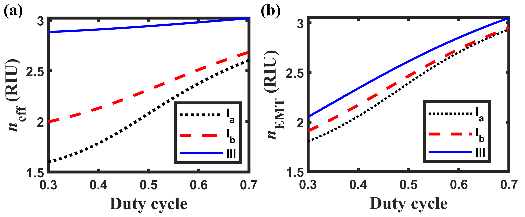
\includegraphics{Fig_sample.pdf}
		\centering
		\caption[Schematic configuration of a conve\ur{n}tional AWG.]
            {\label{fig:1.1}Schematic configuration of a conve\ur{n}tional AWG \cite{awg-fig-2}.}
	\end{figure}
    Blah, Blah, Blah, Blah, Blah, Blah, Blah, Blah, Blah, Blah, Blah, Blah, Blah, Blah, Blah, 
    Blah, Blah, Blah, Blah, Blah, Blah, Blah, Blah, Blah, Blah, Blah, Blah, Blah, Blah, Blah, 
    \begin{figure}[!t]
		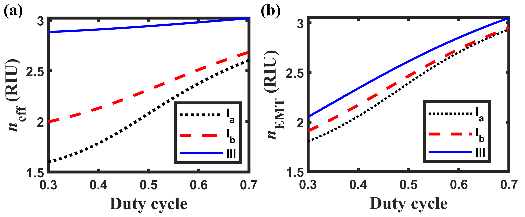
\includegraphics{Fig_sample.pdf}
		\centering
		\caption[Microscope images of an AWG for 1$\times$8 WDM syst\ur{em}]
            {\label{fig:1.2}Microscope images of an AWG for 1$\times$8 WDM syst\ur{em} \cite{awg-fig-2}.}
	\end{figure}
    Blah, Blah, Blah, Blah, Blah, Blah, Blah, Blah, Blah, Blah, Blah, Blah, Blah, Blah, Blah, 
    \begin{figure}[!t]
		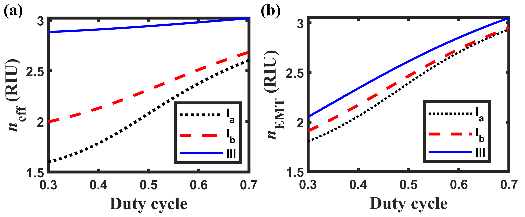
\includegraphics{Fig_sample.pdf}
		\centering
		\caption[SEM images of the AWG shown in Fig.~\ref{fig:1.2}]
            {\label{fig:1.3}SEM images of the AWG shown in Fig.~\ref{fig:1.2} \cite{awg-fig-2}.}
	\end{figure}
    Blah, Blah, Blah, Blah, Blah, Blah, Blah, Blah, Blah, Blah, Blah, Blah, Blah, Blah, Blah, Blah, Blah, Blah, Blah, 
    Blah, Blah, Blah, Blah, Blah, Blah, Blah, Blah, Blah, Blah, Blah, Blah, Blah, Blah, Blah, Blah, Blah, Blah, Blah, 
    Blah, Blah, Blah, Blah, Blah, Blah, Blah, Blah, Blah, Blah, Blah, Blah, Blah, Blah, Blah, Blah, Blah, Blah, Blah, 
    Blah, Blah, Blah, Blah, Blah, Blah, Blah, Blah, Blah, Blah, Blah, Blah, Blah, Blah, Blah, Blah, Blah, Blah, Blah, 
    Blah, Blah, Blah, Blah, Blah, Blah, Blah, Blah, Blah, Blah, Blah, Blah, Blah, Blah, Blah, Blah, Blah, Blah, Blah, 
    Blah, Blah, Blah, Blah, Blah, Blah, Blah, Blah, Blah, Blah, Blah, Blah, Blah, Blah, Blah, Blah, Blah, Blah, Blah.

\subsection{Arrayed waveguide grating (AWG)} \label{sec:1.1.2}
    Blah, Blah, Blah, Blah, Blah, Blah, Blah, Blah, Blah, Blah, Blah, Blah, 
    Blah, Blah, Blah, Blah, Blah, Blah, Blah, Blah, Blah, Blah, Blah, Blah, Blah, Blah, 

% \section{Research motivation and objectives} \label{sec:1.2}

\section{Dissertation configuration} \label{sec:1.2}
    This dissertiation starts with the introduction in Chapter~\ref{chap:1}, illustraing research motivation and objectives. 
    In Chapter~\ref{chap:2}, basic theories for the researches are given, 
    including working principle of AWG (Section~\ref{sec:2.1}), 
    thermal tuning (Section~\ref{sec:2.2}), and WBG (Section~\ref{sec:2.3}).
    For efficient design and analysis of the devices, 
    four solutions including beam propagation method (BPM) (Section~\ref{sec:2.4.1}), 
    heat transport method (Section~\ref{sec:2.4.2}), 
    finite difference eigenmode (FDE) method (Section~\ref{sec:2.4.3}), and 
    finite-difference time-domain (FDTD) method (Section~\ref{sec:2.4.4}) 
    provided by commercial softwares are utilized in the studies, 
    and briefly introduced in the corresponding subsections. 
    
    In Chapter~\ref{chap:3}, 
    a thermally bi-directional tuning feasibility is proposed and demonstrated on an S-shaped AWG 
    at ultra-low voltage using parallel-circuit configuration.
    In Chapter~\ref{chap:4}, 
    a design methodology of WBG is presented to obtain ultra-low XTs and high fabrication tolerance. 
    Moreover, an engineered amplitude apodization based on permittivity-perturbed coupled-mode theory (PPCMT) 
    is employed for accurate evaluation of the resonant wavelength brought by maximum contra-directional coupling coefficient, 
    decreasing the difficulty of designing such devices and the side-lobe imbalance (SLI). 
    At the end of this dissertation, summary and suggestions for future work are given in Chapter~\ref{chap:5}.

% !TeX root = ../main.tex

\chapter{Theoretical Background} \label{chap:2}
\section{Working principle of AWG}\label{sec:2.1}
    \lipsum
    \begin{align}
        \upDelta \lambda_\text{FSR} &= N_\text{ch} \upDelta \lambda\text{,}\label{eq:awg-DFSRLamFSR}\\
        m' &= \frac{\lambda_0}{\upDelta \lambda_\text{FSR}}\text{,}\label{eq:awg-m'}\\
        m &= \text{round}\left(m' \frac{n_{\text{eff}_0}}{N_\ur{\text{g}}}\right)\text{,}\label{eq:awg-m}\\
        N_\text{g} &= n_{\text{eff}_0} - \lambda \frac{\mathrm{d}n_{\text{eff}_0}}{\mathrm{d}\lambda}\text{,}\label{eq:awg-Na}\\
        \upDelta L_\text{0} &= m \frac{\lambda_0}{n_{\text{eff}_0}}\text{,}\label{eq:awg-dL}\\
        f& = R_\text{o} = 2\,R_\text{i} = \frac{n_\text{s}d D}{m' \upDelta \lambda}\text{,}\label{eq:awg-Ro}\\
        D_\text{FSR} &= D\,N_\text{ch}\text{,}\label{eq:awg-DFSR}
    \end{align}
    /lipsum

\section{Working principle of thermal tuning} \label{sec:2.2}
    To date, some thermally tunable AWG leveraging the relation between heat and material refractive indices are implemented on different platforms 
    \cite{TTAWG-p1, TTAWG-p2, TTAWG-p3, TTAWG-n1, TTAWG-n2, TBDTAWG}. 
    Normally, a thermo-optic coefficient of 1.68$\cdot$10\SP{-4}~/K is utilized for silicon layer.
    For more accurate evaluation, two-dimensional (2-D) simulations are performed using the heat transportation 
    followed by the finite-difference eigenmode (FDE) solver 
    to obtain the thermal-diffusion as well as the refractive index change profiles at different electrical voltages. 

\section{Working principle of BGACDC} \label{sec:2.3}
    Recently, 
    a mechanism based on Bragg grating-assisted contra-directional coupling have been used to achieve a flat-top filtering response for CWDM system. 
    To demonstrate the working principle of the device, 
    two concepts including perturbed-permittivity coupled-mode theory (PPCMT) and its anytical expression for brief evaluation of resulting spectrum 
    are geiven in the following two subsections.

\subsection{Coupled-mode theory for permittivity perturbation} \label{sec:2.3.1}
    The differential equations for \ur{Bragg grating-assisted contra-directional coupling} are minimally adjusted 
    based on the perturbed-permittivity coupled-mode theory for fiber Bragg grating presented in \cite{kashyap-fbg}, 
    and given in the following
    \begin{align}
        \frac{\partial B_\text{\textit{\textmu}}}{\partial z} &= j\kappa_\text{dc,\textit{\textmu \textmu}}B_\text{\textit{\textmu}} + 
                j\kappa_\text{ac,\textit{v\textmu}}A_\text{\textit{v}}\cdot \textit{e}^{-j(\upDelta \beta z - \phi (z))}\text{,}\label{eqCMT:1} \\
        \frac{\partial A_\text{\textit{v}}}{\partial z} &= -j\kappa_\text{dc,\ur{\textit{vv}}}A_\text{\textit{v}} - 
                j\kappa_\text{ac,\textit{\textmu v}}B_\text{\textit{\textmu}}
                \cdot \textit{e}^{j(\upDelta \beta z - \phi (z))}\text{,}\label{eqCMT:2}\\
        \kappa_\text{dc,(\textit{vv,\textmu \textmu})} &= \frac{\omega \varepsilon_0}{4} \iint \upDelta \varepsilon_\text{r,dc} (x,y)
            \textbf{E}_\text{\textit{v,\textmu}}(x,y)
            \cdot \textbf{E}_\text{\textit{v,\textmu}}^\text{*}(x,y)\text{d}x\text{d}y\text{,}\label{eqCMT:3} \\
        \kappa_\text{ac,(\textit{v\textmu,\textmu v})} &= \frac{\omega \varepsilon_0}{4} \iint \upDelta \varepsilon_\text{r,ac} (x,y)
            \textbf{E}_\text{\textit{v,\textmu}}(x,y)
            \cdot \textbf{E}_\text{\textit{\textmu ,v}}^\text{*}(x,y)\text{d}x\text{d}y\text{,}\label{eqCMT:4}
    \end{align}
    \lipsum
    
\subsection{Transfer matrix \ur{method}} \label{sec:2.3.2}
    To decribe the contra-directional coupling behavior more clearly with mathematical expression, 
    a transfer matrix in terms of eigenvalue $\alpha_\text{ei}$ is derived as 
    \begin{align}
        \begin{bmatrix}
            R(z) \\
            S(z)
        \end{bmatrix} &= 
        \begin{bmatrix}
            T_\text{11}(z) & T_\text{12}(z) \\
            T_\text{21}(z) & T_\text{22}(z)
        \end{bmatrix}
        \begin{bmatrix}
            R(0) \\
            S(0)
        \end{bmatrix}\text{,}\label{eqCMT:5}\\
        T_\text{11(22)}(z) &= \text{cosh}(\alpha z){\substack{-\\(+)}} j\frac{\delta}{\alpha}\text{sinh}(\alpha z)\text{,}\label{eqCMT:6}\\
        T_\text{12(21)}(z) &= {\substack{-\\(+)}} j\frac{\kappa_\text{ac,\textit{\textmu v}(\textit{v\textmu})}}
        {\alpha}\text{sinh}(\alpha z)\text{,}\label{eqCMT:7}\\
        \delta &= \frac{1}{2}(\kappa_\text{dc,\textit{vv}} + 
                \kappa_\text{dc,\textit{\textmu \textmu}} + \upDelta \beta)\text{,}\label{eqCMT:8}\\
        \upDelta \beta &= \beta_\text{\textit{v}} + \beta_\text{\textit{\textmu}} - \frac{2\pi N}{\Lambda}\text{,}\label{eqCMT:9}\\
        \left|\frac{S(0)}{R(0)}\right|_{S(L)=0}^2 &= \left|\frac{-j\frac{\kappa_\text{ac,\textit{v\textmu}}}{\alpha}\text{sinh}(\alpha L)}
                {\text{cosh}(\alpha L)+j\frac{\delta}{\alpha}\text{sinh}(\alpha L)}\right|^2\text{.}\label{eqCMT:10}
    \end{align}
    \lipsum

\section{Simulation methods} \label{sec:2.4}
    In this section, four solvers/methods are briefly introduced to efficiently design the devices presented in the latter chapters. 
    To evaluate feasibility of a TTAWG, 
    the beam propagation method (BPM), heat transport solver, and FDE solver respectively provided by 
    RSoft and Lumerical are utilized. 
    On the other hand, 
    FDE and finite-difference time-domain (FDTD) are employed to obtain the reflected filtering response of a Bragg grating-assisted structure. 

\subsection{Beam propagation method (BPM)} \label{sec:2.4.1}
    The main concept of BPM \cite{oka-book-bpm} relies on the assumption of dividing electric field $E(x,y,z)$ into two terms including 
    the axially slowly warying envelope term $\phi(x,y,z)$ and the rapid varying phase term exp($-jkn_{0}z$), 
    where $E(x,y,z)$ satisfies the three-dimensional (3-D) scalar wave equation (Helmholtz equation) expressed by 
    \begin{equation}
        \frac{\partial ^2 E}{\partial x^2} + \frac{\partial ^2 E}{\partial y^2} + \frac{\partial ^2 E}{\partial z^2} + 
            k^2 n^2 (x,y,z) E = 0\text{,}\label{eq:Helmholtz}
    \end{equation}
    with the electric field $E(x,y,z)$ equivalent to $\phi(x,y,z)\cdot \text{exp}(-jkn_\text{0}z)$. 
    By the substitution of $E$ into (\ref{eq:Helmholtz}), 
    a formula for BPM can be obtained as 
    \begin{equation}
        \nabla_\text{T}^2 - j2kn_{0}\frac{\partial \phi}{\partial z} + k^2 (n^2 - n_0^2)\phi = 0\text{,}\label{eq:bpm}
    \end{equation}
    where $\nabla_\text{T}^2$ is an operator expressed as 
    \begin{equation}
        \nabla_\text{T}^2 = \frac{\partial^2}{\partial x^2} + \frac{\partial^2}{\partial y^2}\text{.}\label{eq:operator}
    \end{equation}
    To obtain the spatial derivative envelop along the propagation direction, 
    (\ref{eq:bpm}) is utilzied and derived into 
    \begin{equation}
        \frac{\partial \phi}{\partial z} = \frac{-j}{2kn_{\text{EIM}_0}^{}}\frac{\partial^2 \phi}{\partial x^2} - 
            \frac{-jk}{2n_{\text{EIM}_0}^{}}\left[n_\text{EIM}^2 (x,z) - n_{\text{EIM}_0}^2\right]\phi\text{,}\label{eq:bpmz}
    \end{equation}
    where the effective indices $n_{\text{EIM}_0}^{}$ and $n_\text{EIM}^{}$ 
    are the effective indices calculated using effective index method (EIM) 
    to include simulation information within height ($y$) direction. 
    In Chapter~\ref{chap:3}, the BPM provided by RSoft 
    is employed for efficient analysis of the diffractive field as well as beam focusing behavior 
    within the region of two FPRs at different operating wavelengths. 

\subsection{Heat Transport (HT) solver} \label{sec:2.4.2}
    To evaluate heat transport behavior in terms of external electrical sources, 
    three electrical-related equations should be concerened firstly, including 
    (a) the electrical current equation (Ohm's law), 
    (b) the auxiliary continuity equation, and 
    (c) Gauss' law for DC permittivity $\varepsilon$, which can be respectively obtained by 
    \begin{align}
        \textbf{J} = \sigma \textbf{E} = -\sigma \nabla V\text{,}\label{eq:HT1}\\
        \frac{\partial \rho}{\partial t} = -\nabla\cdot\textbf{J}\text{,}\label{eq:HT2}\\
        -\nabla\cdot(\varepsilon \nabla V) = \rho \text{,}\label{eq:HT3}
    \end{align}
    where \textbf{J}, \textbf{E}, $\sigma$, $V$, $\rho$, and $t$ denote 
    current density vector, electrical field vector, electrical conductivity, electrical potential, charge density, and time, respectively. 
    For homogeneous material system, 
    a differential equation can thus be derived into 
    \begin{equation}
        \frac{\partial \rho}{\partial t} + \frac{\sigma}{\varepsilon}\rho = 0\textit{.}\label{eq:HT4}
    \end{equation}
    Under the assumption of quasi-static approximation or steady-state, 
    (\ref{eq:HT1}) combined with (\ref{eq:HT2}) can then reduces into 
    \begin{equation}
        \nabla\cdot(\sigma\textbf{E}) = 0\text{.}\label{eq:HT5}
    \end{equation}
    On the other hand, 
    a $\sigma$-related equation, \textit{i.e.}, 
    power dissipation due to Ohimic loss, can be described by 
    \begin{equation}
        P = \textbf{J}\cdot\textbf{E} = \sigma E^2\text{,}\label{eq:HT6}
    \end{equation}
    and applied to the heat transport equation as a heat energy transfer rate $Q = P$. 
    While Q can be obtained by 
    \begin{equation}
        Q = m_\text{d} C_\text{p} \frac{\partial T}{\partial t} - \nabla \cdot (k_\text{c}\nabla T)\text{,}\label{eq:HT7}
    \end{equation}
    where $m_\text{d}$, $C_\text{p}$, $T$, $t$, and $k_\text{c}$ represent 
    the mass density, the specific heat, temperature, time, and the thermal conductivity, respectively.
    By solving the last three equations (\ref{eq:HT5})--(\ref{eq:HT7}), 
    the heat transportation behavior can be evaluated. 
    In this dissertation, 
    the heat transport (HT) solver provided by Lumerical is utilized to efficiently analyze the thermal tuning problem. 
    % Considering that the thermal-tuning function of TTAWG is introduced by external electrical voltages, 
    % an analysis of heat distributions at different voltages is carried out using heat transport (HT) solver (Lumerical Inc.). 
    % The temperature distributions within a solid medium can be solved over the heat transport equation expressed as 
    % \begin{equation}
        % m_\text{d} C_\text{p} \frac{\partial T}{\partial t} - \nabla \cdot (k_\text{c}\nabla T) = Q\text{,}\label{eq:HT}
    % \end{equation}
    % where $m_\text{d}$, $C_\text{p}$, $k_\text{c}$, and $Q$ represent the mass density, the specific heat, the thermal conductivity, 
    % and the applied heat energy transfer rate, respectively. 
    % Within a homogeneous material region, a differential equation is derived as 
    % \begin{equation}
        % \frac{\partial \rho}{\partial t} + \frac{\sigma \rho}{\varepsilon} = 0\text{,}\label{eq:HTsc}
    % \end{equation}
    % for self-consistent condition with (\ref{eq:HT}).
    % Given that the solution to (\ref{eq:HTsc}) is an exponential decay with a relaxation time $\tau = \varepsilon / \sigma$, 
    % the quasi-static approximation of $\partial \rho / \partial t \sim 0$ can be valid for the time scales of $t \gg \tau$. 
    % In addition, by applying the approximation, 
    % the continuity equation can be reduced into $\nabla\cdot(\sigma \textbf{E}) = \text{0}$.
    % In steady-state with the solution condition $\partial T / \partial t = \text{0}$, 
    % the heat transport equation can be further reduced into 
    % \begin{equation}
        % -\nabla\cdot(k\nabla T) = Q\text{,}\label{eq:HTss}
    % \end{equation}
    % with the electric current equation, again, becoming 
    % \begin{equation}
        % \nabla\cdot(\sigma \textbf{E}) = 0\text{.}\label{eq:HTce}
    % \end{equation}
    % By applying the steady-state HT equation with appropriate finite-element mesh as well as boundary conditions offered by the HT solver, 
    % one can easily evaluate the heat distribution over the modeled region. 
    
\subsection{Finite-difference eigenmode (FDE) solver} \label{sec:2.4.3}
    To solve eigenmode more efficiently, 
    the commercial finite-difference eigenmode (FDE) solver provided by Lumerical is utilized in the following two chapters. 
    During the simulations, 
    the FD algorithm is employed to mesh the waveguide geometry. 
    Maxwell's equations are then formulated into a matrix eigenvalue problem
    which is solved by using sparse matrix technique \cite{lu-fde, fde-oe}. 

\subsection{Finite-difference time-domain (FDTD) solver} \label{sec:2.4.4}
    FDTD, blah, blah, blah, blah, blah, blah, blah, blah, blah, blah, blah, blah, 
    \begin{align}
        \frac{\partial\textbf{B}}{\partial t} &= -\nabla\times\textbf{E} - \textbf{M}\text{,}\label{eq:ME1}\\
        \frac{\partial\textbf{D}}{\partial t} &= \nabla\times\textbf{H}-\textbf{J}\text{,}\label{eq:ME2}\\
        \nabla\cdot\textbf{D} &= \text{0}\text{,}\label{eq:ME3}\\
        \nabla\cdot\textbf{B} &= \text{0}\text{,}\label{eq:ME4}
    \end{align}
    blah, blah, blah, blah, blah, blah, blah, blah, blah, blah, blah, blah, blah, blah, blah, blah, blah, 
    blah, blah, blah, blah, blah, blah, blah, blah, blah, blah, blah, blah, blah, blah, blah, blah, blah, 
    blah, blah, blah, blah, blah, blah, blah, blah, blah, blah, blah, blah, blah, blah, blah, blah, blah, 
    blah, blah, blah, blah, blah, blah, blah, blah, blah, blah, blah, blah, blah, blah, blah, blah, blah, 
    \begin{equation}
        \textbf{J} = \textbf{J}_\text{source}+\sigma \textbf{E};\;\;\;\;
        \textbf{M} = \textbf{M}_\text{source}+\sigma^* \textbf{H}\text{,}\label{eq:JM}
    \end{equation}
    where $\sigma$ and $\sigma^*$ denote electric conductivity and equivalent magnetic loss, respectively, 
    under the condition of linear, isotropic, and nondispersive materials, which can be illustrated by 
    \begin{equation}
        \textbf{D} = \varepsilon\textbf{E} = \varepsilon_\text{r}\varepsilon_\text{0} \textbf{E}\text{;} \;
        \textbf{B} = \mu\textbf{H} = \mu_\text{r}\mu_\text{0}\textbf{H}\text{,}\label{eq:DB}
    \end{equation}
    with $\varepsilon$, $\varepsilon_\text{r}$, $\varepsilon_0$, $\mu$, $\mu_\text{r}$, and $\mu_0$ representing 
    electrical permittivity, relative permittivity, free-space permittivity, 
    magnetic permeability, relative permeability, and free-space permeability, respectively. 
    By the substitution of (\ref{eq:JM}, \ref{eq:DB}) into (\ref{eq:ME1}, \ref{eq:ME2}), 
    two Maxwell's curl equations in linear, isotropic, nondispersive, and lossy materials can be derived as 
    \begin{equation}
        \frac{\partial\textbf{H}}{\partial t} = -\frac{1}{\mu}\nabla\times\textbf{E} - 
            \frac{1}{\mu}\left(\textbf{M}_\text{source}+\sigma^* \textbf{H}\right)\text{;}\;
        \frac{\partial\textbf{E}}{\partial t} = \frac{1}{\varepsilon}\nabla\times\textbf{H} - 
            \frac{1}{\varepsilon}\left(\textbf{J}_\text{source}+\sigma\textbf{E}\right)\text{,}\label{eq:MEfdtdcurl2}
    \end{equation}
    and then six vector components in Cartesian coordinates can be obtained \cite{taflove-book-fdtd} as 
    % \begin{align}
        % \stags
        % \frac{\partial H_x}{\partial t} &= \frac{-1}{\mu}\left[
            % \frac{\partial E_z}{\partial y} - \frac{\partial E_y}{\partial z} + (M_{\text{source}_x}+\sigma^* H_x)
            % \right]\text{,}\tag{\stag}\label{eq:fdtdHx}\\
        % \frac{\partial H_y}{\partial t} &= \frac{-1}{\mu}\left[
            % \frac{\partial E_x}{\partial z} - \frac{\partial E_z}{\partial x} + (M_{\text{source}_y}+\sigma^* H_y)
            % \right]\text{,}\tag{\stag}\label{eq:fdtdHy}\\
        % \frac{\partial H_z}{\partial t} &= \frac{-1}{\mu}\left[
            % \frac{\partial E_y}{\partial x} - \frac{\partial E_x}{\partial y} + (M_{\text{source}_z}+\sigma^* H_z)
            % \right]\text{,}\tag{\stag}\label{eq:fdtdHz}\\
        % \stags
        % \frac{\partial E_x}{\partial t} &= \frac{1}{\varepsilon}\left[
            % \frac{\partial H_z}{\partial y} - \frac{\partial H_y}{\partial z} - (J_{\text{source}_x}+\sigma E_x)
            % \right]\text{,}\tag{\stag}\label{eq:fdtdEx}\\
        % \frac{\partial E_y}{\partial t} &= \frac{1}{\varepsilon}\left[
            % \frac{\partial H_x}{\partial z} - \frac{\partial H_z}{\partial x} - (J_{\text{source}_y}+\sigma E_y)
            % \right]\text{,}\tag{\stag}\label{eq:fdtdEy}\\
        % \frac{\partial E_z}{\partial t} &= \frac{1}{\varepsilon}\left[
            % \frac{\partial H_y}{\partial x} - \frac{\partial H_x}{\partial y} - (J_{\text{source}_z}+\sigma E_z)
            % \right]\text{.}\tag{\stag}\label{eq:fdtdEz}
    % \end{align}
    \begin{align}
        \frac{\partial H_x}{\partial t} = \frac{-1}{\mu}\left[
            \frac{\partial E_z}{\partial y} - \frac{\partial E_y}{\partial z} + (M_{\text{source}_x}+\sigma^* H_x)
            \right]\text{,}
        \frac{\partial E_x}{\partial t} = \frac{1}{\varepsilon}\left[
            \frac{\partial H_z}{\partial y} - \frac{\partial H_y}{\partial z} - (J_{\text{source}_x}+\sigma E_x)
            \right]\text{,}\label{eq:fdtdHx}\\
        \frac{\partial H_y}{\partial t} = \frac{-1}{\mu}\left[
            \frac{\partial E_x}{\partial z} - \frac{\partial E_z}{\partial x} + (M_{\text{source}_y}+\sigma^* H_y)
            \right]\text{,}
        \frac{\partial E_y}{\partial t} = \frac{1}{\varepsilon}\left[
            \frac{\partial H_x}{\partial z} - \frac{\partial H_z}{\partial x} - (J_{\text{source}_y}+\sigma E_y)
            \right]\text{,}\label{eq:fdtdHy}\\
        \frac{\partial H_z}{\partial t} = \frac{-1}{\mu}\left[
            \frac{\partial E_y}{\partial x} - \frac{\partial E_x}{\partial y} + (M_{\text{source}_z}+\sigma^* H_z)
            \right]\text{,}
        \frac{\partial E_z}{\partial t} = \frac{1}{\varepsilon}\left[
            \frac{\partial H_y}{\partial x} - \frac{\partial H_x}{\partial y} - (J_{\text{source}_z}+\sigma E_z)
            \right]\text{.}\label{eq:fdtdHz}
    \end{align}
    
    \begin{figure}[htp]
		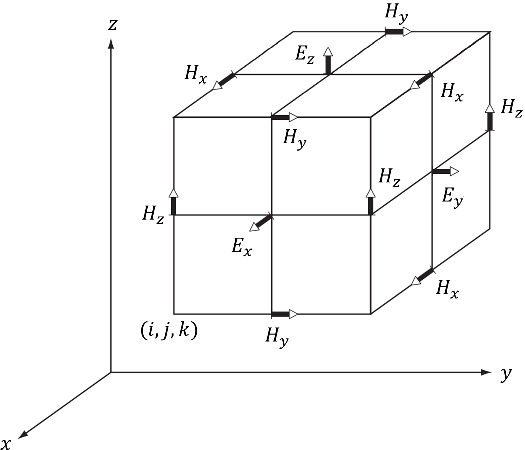
\includegraphics{/YeeCell/YeeCell_300dpi.pdf}
		\centering
		\caption{\label{fig:YeeCell}Yee's Cell for solving time- and space-dependent electric and magnetic fields.}
	\end{figure}
    \clearpage
    \lipsum
    \begin{align}
        \stags
        \begin{split}
            \left. H_x \right\rvert_{i,j+\frac{1}{2},k+\frac{1}{2}}^{n+1} = 
            \left. H_x \right\rvert_{i,j+\frac{1}{2},k+\frac{1}{2}}^{n} 
                &- \frac{\upDelta t}{\mu\upDelta y}
                    \left(\left. E_z\right\rvert_{i,j+1,k+1}^{n+\frac{1}{2}} - 
                        \left. E_z\right\rvert_{i,j,k+1}^{n+\frac{1}{2}}\right) \\
                &+ \frac{\upDelta t}{\mu\upDelta z}
                    \left(\left. E_y\right\rvert_{i,j+\frac{1}{2},k+1}^{n+\frac{1}{2}} - 
                        \left. E_y\right\rvert_{i,j+\frac{1}{2},k}^{n+\frac{1}{2}}\right)\text{,}
        \end{split}\tag{\stag}\label{eq:fdtdgridHx}\\
        \begin{split}
            \left. H_y \right\rvert_{i+\frac{1}{2},j,k+\frac{1}{2}}^{n+1} = 
            \left. H_y \right\rvert_{i+\frac{1}{2},j,k+\frac{1}{2}}^{n} 
                &-\frac{\upDelta t}{\mu\upDelta z}
                    \left(\left. E_x\right\rvert_{i+\frac{1}{2},j,k+1}^{n+\frac{1}{2}} - 
                        \left. E_x\right\rvert_{i+\frac{1}{2},j,k}^{n+\frac{1}{2}}\right) \\
                &+\frac{\upDelta t}{\mu\upDelta x}
                    \left(\left. E_z\right\rvert_{i+1,j,k+\frac{1}{2}}^{n+\frac{1}{2}} - 
                        \left. E_z\right\rvert_{i+1,j,k+\frac{1}{2}}^{n+\frac{1}{2}}\right)\text{,}
        \end{split}\tag{\stag}\label{eq:fdtdgridHy}\\
        \begin{split}
            \left. H_z \right\rvert_{i+\frac{1}{2},j+\frac{1}{2},k}^{n+1} = 
            \left. H_z \right\rvert_{i+\frac{1}{2},j+\frac{1}{2},k}^{n} 
                &-\frac{\upDelta t}{\mu\upDelta x}
                    \left(\left. E_y\right\rvert_{i+1,j+\frac{1}{2},k}^{n+\frac{1}{2}} - 
                        \left. E_y\right\rvert_{i+1,j+\frac{1}{2},k}^{n+\frac{1}{2}}\right) \\
                &+\frac{\upDelta t}{\mu\upDelta y}
                    \left(\left. E_x\right\rvert_{i+\frac{1}{2},j+1,k}^{n+\frac{1}{2}} - 
                        \left. E_x\right\rvert_{i+\frac{1}{2},j+1,k}^{n+\frac{1}{2}}\right)\text{,}
        \end{split}\tag{\stag}\label{eq:fdtdgridHz}\\
        \stags
        \begin{split}
            \left. E_x \right\rvert_{i+\frac{1}{2},j,k}^{n+\frac{1}{2}} = 
            \left. E_x \right\rvert_{i+\frac{1}{2},j,k}^{n-\frac{1}{2}} 
                &+\frac{\upDelta t}{\varepsilon\upDelta y}
                    \left(\left. H_z\right\rvert_{i+\frac{1}{2},j+\frac{1}{2},k}^{n} - 
                        \left. H_z\right\rvert_{i+\frac{1}{2},j-\frac{1}{2},k}^{n}\right) \\
                &-\frac{\upDelta t}{\varepsilon\upDelta z}
                    \left(\left. H_y\right\rvert_{i+\frac{1}{2},j,k+\frac{1}{2}}^{n} - 
                        \left. H_y\right\rvert_{i+\frac{1}{2},j,k-\frac{1}{2}}^{n}\right)\text{,}
        \end{split}\tag{\stag}\label{eq:fdtdgridEx}\\
        \begin{split}
            \left. E_y \right\rvert_{i,j+\frac{1}{2},k}^{n+\frac{1}{2}} = 
            \left. E_y \right\rvert_{i,j+\frac{1}{2},k}^{n-\frac{1}{2}} 
                &+\frac{\upDelta t}{\varepsilon\upDelta z}
                    \left(\left. H_x\right\rvert_{i,j+\frac{1}{2},k+\frac{1}{2}}^{n} - 
                        \left. H_x\right\rvert_{i,j+\frac{1}{2},k-\frac{1}{2}}^{n}\right) \\
                &-\frac{\upDelta t}{\varepsilon\upDelta x}
                    \left(\left. H_z\right\rvert_{i+\frac{1}{2},j+\frac{1}{2},k}^{n} - 
                        \left. H_z\right\rvert_{i-\frac{1}{2},j+\frac{1}{2},k}^{n}\right)\text{,}
        \end{split}\tag{\stag}\label{eq:fdtdgridEy}\\
        \begin{split}
            \left. E_z \right\rvert_{i,j,k+\frac{1}{2}}^{n+\frac{1}{2}} = 
            \left. E_z \right\rvert_{i,j,k+\frac{1}{2}}^{n-\frac{1}{2}} 
                &+\frac{\upDelta t}{\varepsilon\upDelta x}
                    \left(\left. H_y\right\rvert_{i+\frac{1}{2},j,k+\frac{1}{2}}^{n} - 
                        \left. H_y\right\rvert_{i-\frac{1}{2},j,k+\frac{1}{2}}^{n}\right) \\
                &-\frac{\upDelta t}{\varepsilon\upDelta y}
                    \left(\left. H_x\right\rvert_{i,j+\frac{1}{2},k+\frac{1}{2}}^{n} - 
                        \left. H_x\right\rvert_{i,j\frac{1}{2},k+\frac{1}{2}}^{n}\right)\text{.}
        \end{split}\tag{\stag}\label{eq:fdtdgridEz}
    \end{align}
    \clearpage
    In summary, the power coupling behavior between electric and magnetic fields 
    obtained from Maxwell's equations over space and time domain can be described within Yee's cell. 
    By using the central differences for the space derivatives and the leapfrog scheme for the time derivatives, 
    six components ($E_x, E_y, E_z, H_x, H_y, H_z$) of both fields at the specific spatial and 
    the temporal grid can be utilized to evaluate 
    the components at the next grid. 
    In this dissertation, 
    the FDTD solver provided by Lumerical \cite{lu-fdtd} is utilized 
    for efficient analysis as well as the visualization of the 3-D electric and magnetic fields. 
    
% !TeX root = ../main.tex
\clearpage
\setlength{\parskip}{0pt}\chapter{Thermally bi-directionally tunable (TBDT) AWG} \label{chap:3}
    \lipsum

\section{Simulation for passive design} \label{sec:3.1}
    \lipsum

\section{Simulation for active design} \label{sec:3.2}
    \lipsum

\section{Measurement results} \label{sec:3.3}
    \lipsum
    \begin{figure}[!b]
		% \includegraphics[scale = 1.25]{/TBDTAWG/TBDTAWG_Fig7_revised_300dpi.pdf}
        \noindent\makebox[\textwidth]{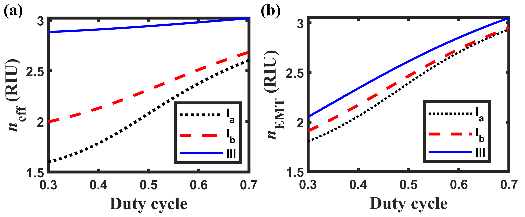
\includegraphics[width=\textwidth]{Fig_sample.pdf}}
		\centering
		\caption{\label{fig:tbdtawgmeadneff_vb}Effective index differences (left y axis) of adjacent AWs and wavelength shifts (right
                                            y axis) of filtering response in terms of electrical voltages at four output Channels 1.27, 1.29,
                                            1.31, and 1.33 \textmu m for \textbf{(a--d)} red-shift tuning and \textbf{(e--h)} blue-shift tuning, 
                                            where the solid line and squared red marker represent the simulated results from Fig.~\ref{fig:tbdtawgsimdneff} 
                                            and the measured data from Fig.~\ref{fig:tbdtawgmeaspec}, respectively.}
	\end{figure}
    \lipsum
    \begin{table}[!b]
		\caption{\label{tab:ttawgcompare}
		Thermal-tuning performance comparison of thermally tunable AWGs in the literature.}
		\centering
		% \begin{ruledtabular}
		% \begin{tabular}{|P{0.6in}|P{0.45in}|P{0.45in}|P{0.45in}|P{0.45in}|P{0.45in}|}	\hline
        %.......................................... For dissertation, total width = 4.75 inches ................................................
        %.......................................... For IEEE journal (two-column), total width = 3.5 inches ..........................
        % \begin{tabular}{|M{0.6in}|M{0.27in}|M{0.25in}|M{0.3in}|M{0.2in}|M{0.3in}|M{0.4in}|}	\hline % well fit for IEEE
		\begin{tabular}{|M{0.76in}|M{0.61in}|M{0.68in}|M{0.76in}|M{0.5in}|M{0.55in}|M{0.89in}|}	\hline % well fit for IEEE
            % \rowcolor{lightgray}\makecell{Literature\textbackslash\\Performance} & 
            \rowcolor{lightgray}\makecell{Literature} & 
            \textcolor{black}{Tuning efficiency} & 
            \textcolor{black}{Tuning direction} & 
            \textcolor{black}{Applied voltage} & 
            \textcolor{black}{Tuning range} & 
            \textcolor{black}{Platform} & 
            \textcolor{black}{TO coefficient} \\ \hline
            
            2020~\cite{TTAWG-p1} & \makecell{6.4\\nm/W} & Red & 40~V for 2.3-nm shift & 
                    2.5~nm & Silicon & 1.68$\cdot 10^{-4}$~/K \\ \hline
            2015~\cite{TTAWG-p3} & \makecell{$\sim$3.97\\nm/W} & Red & 40~V for 5-nm shift & 
                    5~nm & Silicon; SiO$_2$ & \makecell{1.84$\cdot 10^{-4}$~/K;\\1$\cdot 10^{-5}$~/K}\\ \hline
            1999~\cite{TTAWG-n1} & -- & Blue & -- & 
                    9~nm & Polymer & \symbol{"2212}1.6$\cdot 10^{-4}$~/K \\ \hline
            2006~\cite{TTAWG-n2} & -- & Blue & -- & 
                    6.6~nm & Polymer/Si & \symbol{"2212}1.16$\cdot 10^{-4}$~/K \\ \hline
            1999~\cite{TBDTAWG} & \makecell{$\pm2$\\nm/W} & Bi-directional & -- & 
                    6~nm & SiO$_2$--Si & positive \\ \hline
            \textbf{Proposed Device} & \makecell{\textbf{$\pm$30.5}\\nm/W} & \textbf{Bi-directional} & 
                    \textbf{2.5~V for $\pm$8-nm shift} & 
                    \textbf{$\ge\,$8~nm} & Silicon & 1.68$\cdot10^{-4}$~/K \\ \hline
		\end{tabular}
		% \end{ruledtabular}
        % \begin{flushleft}
			% \SP{a} 1-dB bandwidth measured from the transmission peak\\	
			% \SP{b} Available bandwidth (ABW) for channel XT below \symbol{"2212}25~dB\\	
			% \SP{c} Echelle grating; \SP{d} Multi-mode interferometer; \SP{e} Waveguide Bragg grating. \\
		% \end{flushleft}
	\end{table}
    an index change $\upDelta n_\text{eff}$ of $\pm$0.0114 and a shift $\upDelta \lambda$ of $\pm$8~nm 
    are obtained from the measured results,
    indicating a linear bi-directional shift-to-power ratio of $\pm$30.5~nm/W with a wide tuning range
    of 8~nm. The difference of absolute values of linear ratios between simulation (36.07~nm/W)
    and measurement (30.5~nm/W) might come from the power loss in the electrical metal traces or
    from a deviated thickness and/or sheet resistance of the fabricated heating wire. 
    A performance comparison is given in Table~\ref{tab:ttawgcompare}, 
    showing a better thermal-tuning efficiency with bi-directional tuning functions for the proposed device.
    
\section{Discussion} \label{sec:3.4}
    \lipsum

\section{Summary} \label{sec:3.5}
    \lipsum

% !TeX root = ../main.tex

\chapter{Bragg grating-assisted WDM filter} \label{chap:4}
    \lipsum 
    \cite{cwdmf-mmi-3, cwdmf-mmi-1, cwdmf-wbg-1, cwdmf-awgmzi-1, cwdmf-awgmzi-2, cwdmf-awg-5, cwdmf-mzi-9, cwdmf-awg-4, cwdmf-awg-3, cwdmf-mmi-2, cwdmf-mzi-7, cwdmf-wbg-6-1, cwdmf-mzi-3, cwdmf-all, cwdmf-wbg-2, cwdmf-wbg-3, cwdmf-mzi-5, cwdmf-mzi-8, cwdmf-awg-1, cwdmf-wbg-6, cwdmf-eg-1, cwdmf-eg-2, cwdmf-mzi-2, cwdmf-mzi-6, cwdmf-mzi-1, cwdmf-mzi-4, cwdmf-wbg-4, cwdmf-awg-2, cwdmf-wbg-5}. 
    To broaden the available channel bandwidth (ABW) under the desired low crosstalk (XT) 
    to further improve the communication system, flattened filtering responses are required. 
    
    In this chapter, \lipsum

\section{Device structure and optimization} \label{sec:4.1}
    \lipsum
    
    \lipsum
    
    \lipsum
    
    \lipsum
    \ur{Table~\ref{tab:three} shows} performance comparison, 
    \begin{table}[!tb]
		\caption{\label{tab:three}
		Performance comparison of CWDM filters in the literature.}
		\centering
		% \begin{ruledtabular}
		% \begin{tabular}{|M{0.45in}|M{0.27in}|M{0.25in}|M{0.2in}|M{0.3in}|M{0.4in}|M{0.4in}|}	\hline % well fit for IEEE
		\begin{tabular}{|M{.7in}|M{.5in}|M{.5in}|M{.3in}|M{.45in}|M{.6in}|M{.6in}|}	\hline % well fit for IEEE
			\rowcolor{lightgray}\textbf{Structure} & 
            \textbf{EL (dB)} & 
            \textbf{XT (dB)} & 
            \textbf{Mat./ Band} & 
            \textbf{BW\SPSB{a}{1-dB} (nm)} & 
            \ur{\textbf{ABW\SPSB{b}{20-dB} (nm)}} & 
            \ur{\textbf{ABW\SPSB{c}{28-dB} (nm)}} \\ \hline
            
            AWG~\cite{cwdmf-awg-1} (Fig.~6(a)) & 
                    5--6 & \symbol{"2212}27 & InP/ O & 3 & \ur{$<$ 3} & \ur{--} \\ \hline
            AWG~\cite{cwdmf-awg-2} (Fig.~14) & 
                    $\sim$3 & \symbol{"2212}25 & Si/ O & $\sim$11 & \ur{$\sim$12.8} & \ur{--} \\ \hline
            EG\ur{\SP{d}}~\cite{awgeg} (Fig.~5(d)) & 
                    $\sim$3 & \symbol{"2212}2\ur{2} & Si/ C & $\sim$5.7 & \ur{$\sim$7.5} & \ur{--} \\ \hline
            % EG~\cite{cwdmf-eg-1, cwdmf-eg-2} (Fig.~3(c),~3)  & 
            EG~\cite{cwdmf-eg-1} (Fig.~3(c))  & 
                    2--3 & \symbol{"2212}30 & SiN/ O & $\sim$6.7 & \ur{5.7} & \ur{$<$ 3} \\ \hline
            MMI\ur{\SP{e}}~\cite{cwdmf-mmi-2} (Fig.~3(d)) & 
                    2--3 & \symbol{"2212}13 & Si/ C & 8.5 & \ur{--} & \ur{--} \\ \hline
            MMI~\cite{cwdmf-mmi-1} (Fig.~6(b)) & 
                    $<$ 1 & \symbol{"2212}18 & LN/ O & 7.5 & \ur{--} & \ur{--} \\ \hline
            MZI~\cite{cwdmf-mzi-7} (FIg.~6(b)) & 
                    $\sim$0.5 & \symbol{"2212}16 & Si/ C & $\sim$14 & \ur{--} & \ur{--} \\ \hline
            MZI~\cite{cwdmf-mzi-1} (Fig.~5(d)) & 
                    $<$ 1 & \symbol{"2212}23 & Si/ O & 18 & \ur{$\sim$3.7} & \ur{--} \\ \hline
            % MZI (Fig.~3(\ur{b}))~\cite{cwdmf-mzi-9} & 
                    % 1.77 & \symbol{"2212}\ur{20} & SiN/ O & 2.87 & \ur{77} & \ur{--} \\ \hline
            MZI~\cite{cwdmf-mzi-9} (Fig.~3(b)) & 
                    1.78 & \symbol{"2212}15 & SiN/ O & 11.86 & \ur{--} & \ur{--} \\ \hline
            WBG\ur{\SP{f}}~\cite{cwdmf-wbg-6} (Fig.~6(b)) & 
                    $\sim$1 & \symbol{"2212}12 & Si/ C & 12 & \ur{--} & \ur{--} \\ \hline
            WBG~\cite{cwdmf-wbg-1} (Fig.~7) & 
                    $<$ 1 & \symbol{"2212}\ur{13} & Si/ C & 7 & \ur{--} & \ur{--} \\ \hline
            WBG~\cite{cwdmf-wbg-2} (Fig.~5(\ur{c})) & 
                    $\sim$1 & \symbol{"2212}20 & Si/ O & 15 & \ur{$\sim$12} & \ur{--} \\ \hline
            WBG~\cite{cwdmf-wbg-3} (Fig.~5(b)) & 
                    $<$ 1.1 & \symbol{"2212}18 & LN/ C & 10 & \ur{--} & \ur{--} \\ \hline
            \ur{Proposed Structure} & 
                    $<$ \ur{1} & \ur{\textbf{\symbol{"2212}28}} & SiN/ O & \ur{\textbf{13.45}} & \ur{\textbf{$\sim$15.7}} & \ur{\textbf{14.35}} \\ \hline
		\end{tabular}
		% \end{ruledtabular}
        \begin{flushleft}
			\SP{a} 1-dB bandwidth measured from \ur{the} transmission peak.\\	
			\ur{\SP{b} Available bandwidth for channel XT below \symbol{"2212}20~dB, \textit{i.e.}, ABW\SB{20-dB}.}\\	
			\ur{\SP{c}} Available bandwidth for channel XT below \symbol{"2212}2\ur{8}~dB, \textit{i.e.}, ABW\SB{2\ur{8}-dB}.\\	
			\SP{d} Echelle grating; \SP{e} Multi-mode interferometer; \SP{f} Waveguide Bragg grating. \\
		\end{flushleft}
	\end{table}
    \ur{indicating} \ur{the} ultra-low channel XT of \symbol{"2212}28~dB \ur{with its ultra-broad available bandwidth $\sim$14.35~nm}, 
    \ur{outperforming all other CWDM filters in the literature.} 
    % at the cost of \ur{wider} BW\SB{25-dB} (BW\SB{28-dB}).
    %%

\section{Analysis of fabrication tolerance} \label{sec:4.2}
    \lipsum
    
    \lipsum

\section{Summary} \label{sec:4.3}
    \lipsum 
    showing the \ur{great} potential and \ur{high} \ur{attractiveness} of the proposed device \ur{for use in} the 
    \ur{O-band CWDM telecommunication systems}.

% !TeX root = ../main.tex

\chapter{Conclusion} \label{chap:5}
\section{Summary} \label{sec:5.1}
    In this dissertation, 
    \lipsum
    
    In Chapter~\ref{chap:3}, 
    \lipsum
    
    In Chapter~\ref{chap:4}, on the other hand, 
    \lipsum

\section{Suggestion for future work} \label{sec:5.2}
    \lipsum
    
    \lipsum


% 參考文獻
% References
\refmatter
% \bibliographystyle{abbrv}     % ugly format for original template
\bibliographystyle{bibfolder/IEEEtranDOI}     % user-defined bibliography with IEEE, pretty, neat, and comfortable style.
\bibliography{bibfolder/IEEEuabrv, back/references}

% 附錄
% Appendices
% !TeX root = ../main.tex

\appendix{A}{Phase correction for RSoft simulation model}
\section{Introduction}
    Given that the BPM provided by RSoft is utilized with non-rotatable field monitor, 
    a phase-correction step should be involved between two FPRs simulations. 
    The default executable program ``phasecor.exe'' offered by RSoft was replaced with 
    a user-defined python function, 
    considering the wider mode was employed in the AWG to reduce the side-wall roughness. 
    Detailed contents of the python file as well as the mastering callers are provided in the following sections.
\section{phasecor.py}
    TBD
\section{bptmp3Dscanall.bat}
    TBD
\section{bptmp3Dscan1.bat}
    TBD
\section{bptmp3Dout1.bat}
    TBD



% % !TeX root = ../main.tex

\appendix{B}{Adaptive particle swarm algorithm}
\section{Introduction}
    To find the extremum of a figure of merit function more efficiently, 
    an user-defined Lumerical functional script was employed during the optimization of the 
    broadband asymmetric directional coupler with the aim of dropping signal. 
    To meet the Lumerical optmization configuration, 
    three separate scripts named ``APSO\_first.lsf'', ``APSO\_next.lsf'', and ``UDA\_fom'' were developed 
    for ``first generation'', ``next generation'', and ``fom function'' of the optimization. 
\section{APSO\_first}
    TBD
\section{APSO\_next}
    TBD
\section{UDA\_fom}
    TBD
% % !TeX root = ../main.tex

\appendix{C}{Automated python process flow for Lumerical optimization on Taiwania 3 handled by local PC}
\section{Introduction}
    To efficiently perform optimizations under Lumerical over the cloud cluster supercomputer provided by Taiwan government, 
    a user-defined python script allowing for automated actions including 
    logging in, uploading, submitting, monitoring, and downloading jobs was utilized. 
\section{TBD}
    

\end{document}
